%% This work is distributed under the LaTeX Project Public License (LPPL)
%% ( http://www.latex-project.org/ ) version 1.3, and may be freely used,
%% distributed and modified. A copy of the LPPL, version 1.3, is included
%% in the base LaTeX documentation of all distributions of LaTeX released
%% 2003/12/01 or later.
%% Retain all contribution notices and credits.
%% ** Modified files should be clearly indicated as such, including  **
%% ** renaming them and changing author support contact information. **
%%*************************************************************************
\documentclass[conference]{IEEEtran}
%%%%%%%%%%%%%%%%%%%%%%%%%%%%%%%%%%%%%%%%%%%%%%%%%%%%%%%%%%%%%%%%%%%%%%%%%%%%%%%%
%%
%% Преамбула
%%
%%%%%%%%%%%%%%%%%%%%%%%%%%%%%%%%%%%%%%%%%%%%%%%%%%%%%%%%%%%%%%%%%%%%%%%%%%%%%%%%
\documentclass[%
  a5paper,
  subf,
  href,
  master,
  dotsinheaders
]{csse-fcs}

\usepackage[T2A]{fontenc}
\usepackage[utf8]{inputenc}
\usepackage[english,russian]{babel}
 
% Компактные списки
\usepackage{mdwlist}

% Таблицы
\usepackage{array}

% Листинги
\usepackage{listings}

% TODOs
\usepackage[%
  colorinlistoftodos,
  shadow
]{todonotes}

% Путь к каталогу со всеми рисунками
\graphicspath{{fig/}}

% Автоконвертер для EPS
\usepackage{epstopdf}

% Генератор текста
\usepackage{blindtext}

%%%%%%%%%%%%%%%%%%%%%%%%%%%%%%%%%%%%%%%%%%%%%%%%%%%%%%%%%%%%%%%%%%%%%%%%%%%%%%%%


%% Bibliography file
\addbibresource{seim.bib}


% If you need to correct hyphenations, add them here
\hyphenation{op-tical net-works semi-conduc-tor}


\begin{document}
%
% paper title
%
% In English titles are generally capitalized except for words such as a, an, and, as,
% at, but, by, for, in, nor, of, on, or, the, to and up, which are usually
% not capitalized unless they are the first or last word of the title.
% Linebreaks \\ can be used within to get better formatting as desired.
% Do not put math or special symbols in the title.
\title{Разработка аспектно-ориентированного расширения для языка Kotlin}


% author names and affiliations
% use a multiple column layout for up to three different
% affiliations
\author{\IEEEauthorblockN{Борис Скрипаль}
\IEEEauthorblockA{Санкт-Петербургский политехнический \\университет Петра
Великого\\
Email: skripal@kspt.icc.spbstu.ru}
\and
\IEEEauthorblockN{Владимир Ицыксон}
\IEEEauthorblockA{Санкт-Петербургский политехнический \\университет Петра
Великого\\
Email: vlad@icc.spbstu.ru}
}

% make the title area
\maketitle

%%%%%%%%%%%%%%%%%%%%%%%%%%%%%%%%%%%%%%%%%%%%%%%%%%%%%%%%%%%%%%%%%%%%%%%%%%%%%%%%
\begin{abstract}
%%%%%%%%%%%%%%%%%%%%%%%%%%%%%%%%%%%%%%%%%%%%%%%%%%%%%%%%%%%%%%%%%%%%%%%%%%%%%%%%

В статье описывается разработка аспектно-ориентированного расширения для языка
Kotlin.
Представлен краткий обзор существующих на данный момент аспектно-ориентированных
расширений для различных объектно-ориентированных языков программирования,
проанализированы различные способы внедрения аспектов.
Разрабатывается программный прототип, позволяющий использовать
аспектно-ориентированный подход при написании программ на языке Kotlin,
проектируется язык описания аспектов.
Созданный прототип протестирован на серии примеров.
Тестирование показало корректность предложенного подхода и работоспособность
прототипа.
%%%%%%%%%%%%%%%%%%%%%%%%%%%%%%%%%%%%%%%%%%%%%%%%%%%%%%%%%%%%%%%%%%%%%%%%%%%%%%%%
\end{abstract}
%%%%%%%%%%%%%%%%%%%%%%%%%%%%%%%%%%%%%%%%%%%%%%%%%%%%%%%%%%%%%%%%%%%%%%%%%%%%%%%%

%%%%%%%%%%%%%%%%%%%%%%%%%%%%%%%%%%%%%%%%%%%%%%%%%%%%%%%%%%%%%%%%%%%%%%%%%%%%%%%%
\section{Введение}
%%%%%%%%%%%%%%%%%%%%%%%%%%%%%%%%%%%%%%%%%%%%%%%%%%%%%%%%%%%%%%%%%%%%%%%%%%%%%%%%

Аспектно-ориентированный подход (АОП) был предложен как решение проблемы
описания сквозной функциональности в объектно-ориентированных программах.
Впервые подход был представлен в 1997 году Грегором Кичалесом в работе
<<Aspect-oriented programming>>~\cite{kiczales_aop}.
В предложенном подходе, сквозная функциональность описывается отдельно от
объектно-ориентированного кода программы и внедряется на этапе компиляции.
Такое разделение позволяет не только компактно описывать сквозную 
функциональность, но и делать её внедрение прозрачным для программиста.

Парадигма АОП предложила элегантное решение для ряда задач, как, например, 
протоколирование и трассировка программ, работа с транзакциями, обработка
ошибок, а также некоторых других.
АОП стал интенсивно развиться и, в настоящий момент, аспектно-ориентированные
расширения созданы для большинства объектно-ориентированных языков
программирования, как, например, C++, C\#, Java, Python и т.п.

В данной статье мы представляем аспектно-ориентированное расширение для нового 
языка программирования Kotlin.
Язык Kotlin --- молодой мультипарадигменный язык программирования,
разрабатываемый компанией JetBrains.
Основная цель языка Kotlin быть компактной, выразительной и надежной заменой
языка Java.
При этом язык обеспечивает полную интероперабельность с программами на языке
Java.

Наличие существенного числа новых конструкций не позволяет использовать уже 
готовые АОП-расширения для JVM-совместимых языков, поэтому
аспектно-ориентированное  расширение для языка Kotlin необходимо разрабатывать,
специально ориентируясь на особенности языка Kotlin. 

Оставшаяся часть статьи организована следующим образом. 
В втором разделе приведено общее описание аспектно-ориентированной парадигмы, 
в третьем разделе представлены актуальные реализации аспектно-ориентированных 
расширений.
Четвертый раздел посвящен описанию разрабатываемого расширения для языка Kotlin.
В пятом разделе проводится тестирование расширения на реальных проектах.
В заключении приводятся направления дальнейшего развития. 

% Одним из главных принципов объектно-ориентированного программирования является
% инкапсуляция - сокрытие данных и методов, работающих с этими данными, в
% некоторых сущностях - классах.
% При таком подходе данные и функциональность, работающая с этими данными,
% локализованы в отдельном месте, что позволяет создавать абстракцию, с которой
% удобно манипулировать для создания больших и сложных программ.
% Однако, существует функциональность, называемая сквозной функциональностью, не
% привязанная к конкретному месту в программе, а, наоборот, рассредоточенная по
% всей программе, в связи с чем она плохо описывается при использовании
% объектно-ориентированного подхода.
% В 1997 году данная проблема была описана Грегором Китчзалесом в своей работе
% <<Aspect-oriented programming>>~\cite{kiczales_aop}.
% Также в данной работе был предложен аспектно-ориентированный подход, который
% удобно описывал сквозную функциональность при написании программ в
% объектно-ориентированном стиле.

% При использовании аспектно-ориентированного подхода, сквозная функциональность
% инкапсулируется в отдельные сущности - советы (<<advices>>), которые являются
% частью более большей сущности - аспекта (<<aspect>>).
% Помимо этого, аспекты содержат описания срезов (<<pointcuts>>), по которым
% происходит поиск точек соединения (<<join points>>), к которым уже применяется
% сквозная функциональность, описанная в советах.
% Данный подход позволяет описывать сквозную функциональность и места её внедрения
% отдельно от объектно-ориентированного кода программы, и делать её применение
% прозрачным для разработчика.
%%%%%%%%%%%%%%%%%%%%%%%%%%%%%%%%%%%%%%%%%%%%%%%%%%%%%%%%%%%%%%%%%%%%%%%%%%%%%%%%

%%%%%%%%%%%%%%%%%%%%%%%%%%%%%%%%%%%%%%%%%%%%%%%%%%%%%%%%%%%%%%%%%%%%%%%%%%%%%%%%
\section{Аспектно-ориентированный подход}
%%%%%%%%%%%%%%%%%%%%%%%%%%%%%%%%%%%%%%%%%%%%%%%%%%%%%%%%%%%%%%%%%%%%%%%%%%%%%%%%

При использовании АОП, сквозная функциональность инкапсулируется в отдельные 
сущности, называемые \textit{аспектами}.
Каждый аспект состоит из \textit{советов} и \textit{срезов}. 
Совет --- сущность, содержащая в себе непосредственно сквозную функциональность
(код совета), а также способ её внедрения в программный код.
Срез --- описание множества \textit{точек внедрения} советов. 
Типовыми способами внедрения сквозной функциональности являются:
\begin{itemize}
     \item вставка совета до точки внедрения;
     \item вставка совета после точки внедрения;
     \item вставка совета после возникновения исключительной ситуации;
     \item вставка совета вместо точки внедрения.
\end{itemize}

% Как было сказано выше, аспект содержит в себе не только описание сквозной
% функциональности, но и правила её применения (построения срезов).
% При описании срезов, как правило, используются следующее:
% \begin{itemize}
%     \item вызов некоторого метода;
%     \item исполнение некоторого метода;
%     \item возникновение исключительной ситуации;
%     \item поток управления среза.
% \end{itemize}

% Совет, в свою очередь, содержит две составные части: сквозную функциональность
% и место её внедрения, относительно точки включения.
% Как правило, в большинстве аспектно-ориентированных расширений реализовываются
% следующие места внедрения:
% \begin{itemize}
%     \item вставка кода совета перед точкой включения;
%     \item вставка кода совета после точки включения;
%     \item вставка кода совета до и после точки включения;
%     \item вставка кода совета после возвращения;
%     \item вставка кода совета вместо точки включения;
%     \item вставка кода совета после возникновения исключительной ситуации.
% \end{itemize}

Вставка кода совета может производиться статически и динамически.
При статическом способе внедрения советов, сквозная функциональность внедряется
или на этапе сборки (модификация исходных кодов программы и модификация
промежуточного представления в процессе компиляции), или же, сразу после сборки, 
например, путем модификации байт-кода.
Основным преимуществом данного подхода является высокое быстродействие, однако, 
при изменении одного совета, будет необходима повторная сборка всего проекта.

При динамическом внедрении сквозной функциональности код советов применяется
непосредственно в процессе выполнения программы.
Одним из способов динамического внедрения советов является создание 
прокси-объектов~\cite{aspect_dynamic_weavers}, которые перехватывают
исполнение программы, позволяя выполнять код совета до, после или вместо точки
внедрения.
Такой способ внедрения аспектов не требует повторной сборки всего проекта после
изменения аспектов, однако имеет меньшую производительность.
%%%%%%%%%%%%%%%%%%%%%%%%%%%%%%%%%%%%%%%%%%%%%%%%%%%%%%%%%%%%%%%%%%%%%%%%%%%%%%%%

%%%%%%%%%%%%%%%%%%%%%%%%%%%%%%%%%%%%%%%%%%%%%%%%%%%%%%%%%%%%%%%%%%%%%%%%%%%%%%%%
\section{Обзор существующих аспектно-ориентированных расширений}
%%%%%%%%%%%%%%%%%%%%%%%%%%%%%%%%%%%%%%%%%%%%%%%%%%%%%%%%%%%%%%%%%%%%%%%%%%%%%%%%

Перед разработкой АОП-расширения для языка Kotlin рассмотрим существующие на
рынке АОП-решения и их основные особенности.
%%%%%%%%%%%%%%%%%%%%%%%%%%%%%%%%%%%%%%%%%%%%%%%%%%%%%%%%%%%%%%%%%%%%%%%%%%%%%%%%

\subsection{AspectJ}
%%%%%%%%%%%%%%%%%%%%%%%%%%%%%%%%%%%%%%%%%%%%%%%%%%%%%%%%%%%%%%%%%%%%%%%%%%%%%%%%
AspectJ --- первое аспектно-ориентированное расширение для языка Java, оно 
было представлено в 2003 году~\cite{kiczales_aspectj} и развивается до сих 
пор\footnote{На момент написания статьи последняя доступная версия 1.8.10 
датирована 12 декабря 2016г.}.
AspectJ расширяет грамматику языка Java, предоставляя дополнительные языковые
конструкции для описания аспектов.
В отличие от классов описание аспекта в AspectJ начинается с ключевого слова
\textit{aspect}. Сам аспект имеет уникальное имя и состоит из тела, которое 
содержит описание срезов и советов, а также может использовать переменные и 
методы языка Java.
Описания срезов могут задаваться как отдельно от совета (в таком случае им
необходимо задавать идентификатор, уникальный в рамках аспекта), так и,
непосредственно, при описании совета.
Способ внедрения кода совета относительно точки объединения задается при
описании совета с помощью ряда ключевых слов: \textit{before} (после точки
объединения), \textit{after} (перед точкой объединения) и т.д.

AspectJ поддерживает статический и динамический способы внедрения аспектов~
\cite{aspectj_doc}.
Статическое внедрение аспектов может производиться, как на уровне исходных
кодов, так и сразу после компиляции программы (внедрение кода советов в байт-код
скомпилированной программы).
Динамическое внедрение аспектов производится непосредственно перед тем, как JVM
загружает файл класса, что позволяет увеличить производительность, по сравнению
с использованием прокси-объектов.

%%%%%%%%%%%%%%%%%%%%%%%%%%%%%%%%%%%%%%%%%%%%%%%%%%%%%%%%%%%%%%%%%%%%%%%%%%%%%%%%

%%%%%%%%%%%%%%%%%%%%%%%%%%%%%%%%%%%%%%%%%%%%%%%%%%%%%%%%%%%%%%%%%%%%%%%%%%%%%%%%
\subsection{SpringAOP}
%%%%%%%%%%%%%%%%%%%%%%%%%%%%%%%%%%%%%%%%%%%%%%%%%%%%%%%%%%%%%%%%%%%%%%%%%%%%%%%%

Другим популярным АОП-расширением для языка Java является SpringAOP ---
расширение, входящее в состав фреймворка <<Spring Framework>>.
Первая версия данного расширения была представлена в 2005 году, последняя
 (5.0.0.M5) - в феврале 2017 года.
Для описания аспектов в SpringAOP используются специальные аннотации,
размечающие классы и их методы, как аспекты, советы и срезы
~\cite{springAOP_doc}.
Также, как и в AspectJ, аспект может содержать не только описание срезов или
советов, но и обычные в понимании языка Java переменные и методы.
% SpringAOP имеет чуть более бокатый синтаксис для описания срезов и советов~
% \cite{springAOP_doc}.
% Срезы могут описываться при помощи таких же правил, что и в AspectJ, но для
% удобства было введено еще несколько правил:
% \begin{itemize}
%     \item annotation(Имя\_аннотации) - задает точки соединения для методов,
%           имеющих соответствующую аннотацию;
%     \item bean(Имя) - срез формируется из бинов, чье имя или идентификатор
%           совпадают с заданной маской.
% \end{itemize}
% Также, введено два дополнительных способа внедрения кода совета:
% \begin{itemize}
%     \item around - вставить код совета до и после точки объединения;
%     \item after finally - выполнить код совета после точки объединения, вне
%           зависимости от того, была ли исключительная ситуация или нет.
% \end{itemize}

% Для описания аспектов, в SpringAOP используется механизм аннотаций: сам аспект
% представляется, как обычный класс на языке Java с аннотацией.
% В листинге~\ref{springAOP_aspect_ex} приведен пример описания аспектов:
% \begin{lstlisting}[label=springAOP_aspect_ex,
%     caption={Пример объявления аспекта в расширении SpringAOP}]
% @Aspect
% public class A {
%     @Before("execution(Foo.foo()) && call(println(String))")
%     public void advEx() {
%         System.out.println("Bar");
%     }
% }
% \end{lstlisting}

SpringAOP поддерживает только динамическое внедрение аспектов в код.
Основным способом применение аспектов в SpringAOP является связывание при
помощи прокси-объектов.
%Также в SpringAOP существует совместимость с AspectJ и, вследствие, существует
%возможность применения советов при загрузке файлов в JVM.
% * <vlad@icc.spbstu.ru> 11:13:41 19 Mar 2017 UTC+0300:
% Последняя фраза написана очень плохо: "существует совместимость". Может вообще об этом не писать?

%%%%%%%%%%%%%%%%%%%%%%%%%%%%%%%%%%%%%%%%%%%%%%%%%%%%%%%%%%%%%%%%%%%%%%%%%%%%%%%%

%%%%%%%%%%%%%%%%%%%%%%%%%%%%%%%%%%%%%%%%%%%%%%%%%%%%%%%%%%%%%%%%%%%%%%%%%%%%%%%%
\subsection{PostSharp}
%%%%%%%%%%%%%%%%%%%%%%%%%%%%%%%%%%%%%%%%%%%%%%%%%%%%%%%%%%%%%%%%%%%%%%%%%%%%%%%%

Еще одной реализацией АОП является PostSharp --- АОП-фреймворк для программ, 
написанных на языке C\#.
PostSharp было представлен в 2004 году~\cite{postsharp_doc}, как свободная
библиотека для языка C\#, однако, в 2009 году данное расширение стало
проприетарным.
На момент написания статьи, последняя стабильная версия расширения 4.3.29 была
представлена в феврале 2017 года.
Для описания аспектов, в PostSharp существует ряд классов, обеспечивающих
внедрения кода совета в программу.
Каждый из таких классов определяет некоторый набор способов включения сквозной
функциональности относительно точки объединения~\cite{postsharp_aspects}.
Для реализации аспектов, необходимо переопределить соответствующие методы этого
класса, а также прописать правила формирования среза внутри специальных
аннотаций данного класса.
% Основными классами~\cite{postsharp_aspects} являются:
% \begin{itemize}
%     \item OnMethodBoundaryAspect - класс, позволяющий отслеживать начало и конец
%           вызова метода, а также возникновение исключительных ситуаций и
%           нормальное завершение метода.
%           Для того, чтобы применить совет, необходимо переопределить методы
%           OnEntry, OnExit, OnException и OnSuccess, соответственно.
%     \item LocationLevelAspect - класс, позволяющий отслеживать обращения к полям
%           классов.
%           Для того, чтобы перехватить обращение за чтением, необходимо
%           переопределить метод OnGetValue и для записи - OnSetValue.
%     \item OnExceptionAspect  - данный метод вставляет обработчик исключений в
%           метод, к которому применен аспект.
%           При помощи переопределения метода GetExceptionType  можно задать какие
%           типы исключений будут перехватываться (по умолчанию перехватываются
%           все типы исключений).
%           Обработчик исключений переопределяется в методе OnException.
% \end{itemize}

PostSharp поддерживает как статический, так и динамический способы внедрения
аспектов.
Для динамического применения аспектов могут использоваться как прокси-объекты,
так и перехват момента загрузки файла в память, после чего аспекты применяются
непосредственно к бинарному файлу.
Статическое внедрение аспектов может производиться как на уровне исходных кодов,
так и во время компиляции.
При применении аспектов во время компиляции используется MSIL --- промежуточное
представление, создаваемое в процессе компиляции программ для платформы .NET.
MSIL является независимым от процессора набором инструкций, который впоследствии
преобразуется в набор кодов для конкретного процессора.
Такой подход позволяет удобно анализировать целевую программу, а также
избавляет от необходимости поддерживать корректность исходных кодов программы
после внедрения аспектов, что необходимо делать при модификации на уровне
исходных кодов.
% * <vlad@icc.spbstu.ru> 11:16:55 19 Mar 2017 UTC+0300:
% Сюда вы общий вывод для всего раздела

%%%%%%%%%%%%%%%%%%%%%%%%%%%%%%%%%%%%%%%%%%%%%%%%%%%%%%%%%%%%%%%%%%%%%%%%%%%%%%%%

По результатам анализа ряда популярных АОП-расширений можно сделать вывод о том,
что не смотря на схожую функциональность, расширения сильно отличаются как
способами описания аспектов, так и способами их внедрения.
Данные различия обусловлены не только особенностями языка
программирования, для которого предназначено расширение, но и стремлением
сделать синтаксис описания аспектов как можно более удобным и понятным для
разработчика.

%%%%%%%%%%%%%%%%%%%%%%%%%%%%%%%%%%%%%%%%%%%%%%%%%%%%%%%%%%%%%%%%%%%%%%%%%%%%%%%%

%%%%%%%%%%%%%%%%%%%%%%%%%%%%%%%%%%%%%%%%%%%%%%%%%%%%%%%%%%%%%%%%%%%%%%%%%%%%%%%%
\section{Разработка аспектно-ориентированного расширения для языка Kotlin}
%%%%%%%%%%%%%%%%%%%%%%%%%%%%%%%%%%%%%%%%%%%%%%%%%%%%%%%%%%%%%%%%%%%%%%%%%%%%%%%%

При реализации аспектно-ориентированного расширения необходимо сформировать
синтаксис аспектов и определить механизмы внедрения аспектов.

%%%%%%%%%%%%%%%%%%%%%%%%%%%%%%%%%%%%%%%%%%%%%%%%%%%%%%%%%%%%%%%%%%%%%%%%%%%%%%%%
\subsection{Разработка синтаксиса описания аспектов}
%%%%%%%%%%%%%%%%%%%%%%%%%%%%%%%%%%%%%%%%%%%%%%%%%%%%%%%%%%%%%%%%%%%%%%%%%%%%%%%%

Описание аспектов является расширением языка программирования и должно позволять
в удобной и понятной форме задавать все сущности АОП: аспекты, советы, срезы и
т.п.
В этой работе мы приняли решение не разрабатывать специализированный синтаксис 
аспектов для языка Kotlin, а воспользоваться возможностями  AspectJ для 
языка Java, расширив его необходимыми для языка Kotlin конструкциями. 
Такой выбор был сделан по нескольким причинам:
\begin{itemize}
	\item синтаксис описания аспектов, используемый в AspectJ, является очень
		  удобным для программиста;
	\item грамматика AspectJ, описанная на языке ANTLR4, находится
		  в свободном доступе и может быть использована для разработки
		  языка аспектов для языка Kotlin;
	\item AspectJ является одним из самых популярных аспектно-ориентированных
		  расширений для языка Java~\cite{aspect_review} и знаком многим
		  разработчикам.
\end{itemize}

%%TODO список изменений синтаксиса aspectj
Для адаптации AspectJ к языку Kotlin в синтаксис AspectJ были внесены следующие
изменения:
\begin{itemize}
	\item способ описания методов был изменен в соответствии с правилами языка
	      Kotlin;
	\item стандартные типы языка Java были заменены на стандартные типы языка
		  Kotlin;
	\item в соответствии с правилами языка Kotlin изменены модификаторы полей и
	      методов;
	\item добавлена возможность задавать атрбуты аргументов методов;
	\item добавлена поддержка функций-расширений (extension functions).
\end{itemize}

Описание аспекта начинается с ключевого слова \textit{aspect} и состоит из 
идентификатора аспекта и тела аспекта.
Тело аспекта может содержать в себе описание срезов и советов.
Описание среза начинается с ключевого слова \textit{pointcut} и состоит из
идентификатора среза и правила, в соответствии с которым производится
формирования среза.

Правило формирование среза по сути является описанием множества точек включения, 
для задания которого используются логические операции и специальные ключевые 
слова, например, \textit{execution} или \textit{call}, указывающие на
определенную группу мест в программном коде.
Допускается описывать одни срезы с использованием других. 

Для указания множества методов, входящих в срез, используются следующие
механизмы:
\begin{itemize}
    \item модификаторы видимости с логическими операторами (например, можно
          выделить все не public методы);
    \item класс, к которому принадлежит метод;
    \item имя метода или его часть;
    \item список аргументов метода с атрибутами;
    \item тип возвращаемого значения.
\end{itemize}
Описание совета состоит из описания способа применения совета (например,
\textit{before} или \textit{after}), правила формирования среза и кода совета.

Пример описания аспекта приведен в листинге~\ref{prototype_aspect_ex}.
\begin{lstlisting}[label=prototype_aspect_ex,
    caption={Пример описания аспекта}]
aspect A  {
    pointcut fooPC(): execution(fun Foo.*())
    pointcut printPC(): call(public fun kotlin.io.pri*(!Any))

    after(): fooPC() && printPC() {
        println("Hello after!!")
    }

    before(): fooPC() && printPC() {
        println("Hello before!!")
    }
}
\end{lstlisting}
Приведенный в листинге аспект содержит описание двух срезов: fooPC и printPC.
Срез fooPC включает в себя все места вызовов функций и инициализации переменных
внутри всех методов класса Foo.
% * <vlad@icc.spbstu.ru> 08:23:52 17 Mar 2017 UTC+0300:
% Какие точки? Надо переформулировать
Срез printPC включает в себя все места вызовов публичных методов пакета
kotlin.io, имя которых начинается с pri, принимающих один аргумент, тип
которого отличается от Any.
Далее описываются два совета: первый вставляет код совета (вызов метода println) 
до всех точек включения, которые принадлежат одновременно к двум срезам fooPC и
printPC, второй --- после.
После применения совета к программе, во всех местах вызовов методов,
удовлетворяющих следующим условиям:
\begin{itemize}
	\item вызов происходит внутри методов, принадлежащих классу Foo;
	\item вызываемый метод имеет модификатор public и принадлежит к пакету
		  kotlin.io;
	\item имя вызываемой метода начинается с pri;
	\item метод принимает единственный аргумент, тип которого отличается от
	      <<Any>>.
\end{itemize}
 до вызова метода будет выведена на печать строка <<Hello after!!>>, а после ---
<<Hello before!!>>.
% * <vlad@icc.spbstu.ru> 08:32:26 17 Mar 2017 UTC+0300:
% В этом разделе необходимо описать те расширения, которые мы сделали для Котлина или те изменения, которые мы внесли в исходный язык.

%%%%%%%%%%%%%%%%%%%%%%%%%%%%%%%%%%%%%%%%%%%%%%%%%%%%%%%%%%%%%%%%%%%%%%%%%%%%%%%%

%%%%%%%%%%%%%%%%%%%%%%%%%%%%%%%%%%%%%%%%%%%%%%%%%%%%%%%%%%%%%%%%%%%%%%%%%%%%%%%%
\subsection{Внедрение аспектов}
%%%%%%%%%%%%%%%%%%%%%%%%%%%%%%%%%%%%%%%%%%%%%%%%%%%%%%%%%%%%%%%%%%%%%%%%%%%%%%%%

Язык Kotlin имеет ряд оригинальных языковых конструкций (extension функции,
специфичные лямбда-функции и т.п.), при этом основной целевой платформой
компиляции для языка Kotlin является JVM.
Как результат --- все специальные конструкции Kotlin преобразуются в стандартный
байт-код, который имеет одинаковую структуру и для Java, и для Kotlin-программ.
Из-за этого поиск некоторых структур языка Kotlin в байт-коде становится
затруднительным и, как следствие, динамическое внедрение кода советов при
загрузке файлов в JVM становится практически невозможным.
По той же причине статическое внедрение советов в байт-код программы также
является очень сложной задачей.

Таким образом, единственным разумным способом внедрения аспектов является
внедрение аспектов в исходный код программы или в модель программы во время
компиляции. 

Разработчики языка Kotlin предусмотрели специальную структуру данных для работы
с программным кодом --- Program Structure Inteface (PSI).
В нашем проекте мы используем PSI для внедрения объектов на этапе компиляции
проекта. 

%Так как при внедрении советов в исходный код программы необходимо собственноручно
%составлять модель программы, было решено модифицировать промежуточное
%представление, создаваемое в процессе компиляции проекта.
%При этом, работа по составлению модели программы перекладывается на компилятор
%языка Kotlin, а также отпадает необходимость удаления кода советов из исходных
%кодов после компиляции программы.

% Перед проектированием части, отвечающей за внедрения, необходимо выбрать способ
% применения аспектов.
% Как было сказано ранее, все способы внедрения можно разделить на две группы:
% статический и динамический способы применения аспектов.
% Для динамического внедрения, как правило, используются два подхода: внедрение
% при помощи прокси-объектов или же внедрение во время загрузки классов в JVM.
% Применение аспектов при помощи прокси-объектов было отвергнуто ввиду того, что
% данный подход замедляет выполнение программы, а также достаточно сложен в
% реализации.
% Применение советов во время загрузки файлов классов в JVM не представляется
% возможным, так как при компиляции программы на языке Kotlin в байт код теряется
% часть особенностей языка
% Kotlin (например extended функции), невозможно выделить,
% анализируя байт-код программы.

% Статическое внедрение аспектов для программ, работающих поверх JVM может быть
% выполнено одним из трех способов: модификация исходных кодов программы перед
% компиляцией программы, внедрение аспектов во время компиляции, или же сразу
% после компиляции путем модификации байт-кода.
% Внедрение аспектов непосредственно в байт-код программы была отвергнута по
% причинам, указанным выше.
% При модификации исходного кода возникает необходимость приведения кода в
% изначальное состояние после компиляции программы, а также необходимость
% построения модели программы, что является хоть и разрешимой, однако, трудоемкой
% задачей.

% Для реализации аспектно-ориентированного расширения было решено использовать
% статический способ внедрения аспектов, а, если быть точнее, внедрение аспектов
% в момент формирования промежуточного представления программы в процессе
% компиляции программы.
% Данный способ внедрения сквозной функциональности был выбран из-за того, что
% промежуточное представление программы, создаваемое компилятором языка легче
% анализировать, чем исходные файлы программы, а также при модификации
% промежуточного представления отпадает необходимость поддерживать корректность
% исходных кодов программы.

Внедрение аспектов происходит в несколько этапов, схематически изображенных на
рисунке~\ref{fig:aspect_weaving}.
\begin{figure*}[!t]
\centering
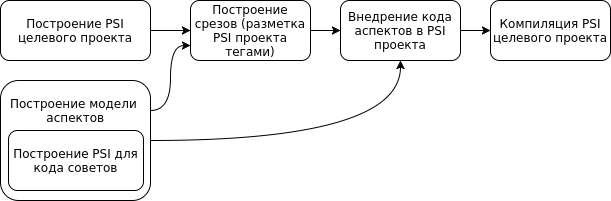
\includegraphics[width=0.8\textwidth]{aspect_weaving}
\caption{Процесс внедрения аспектов в программный код при компиляции}
\label{fig:aspect_weaving}
\end{figure*}

Первым этапом является построение PSI --- промежуточного представления проекта, 
состоящего из набора виртуальных файлов, соответствующих исходными файлам, а 
также из прочей информации о проекте (конфигурация, путь до JDK и т.п.).
Каждый из этих файлов содержит дерево разбора программного кода и информацию о
файле.
Каждый элемент дерева разбора содержит в себе текст соответствующего элемента,
ссылки на потомков и различную сопровождающую информацию.
Одним из таких полей является <<userMap>> типа \textit{KeyFMap} --- структура в,
которую могут быть записаны различные пользовательские данные.
На рисунке~\ref{fig:aspect_weaving} схематически представлен процесс внедрения
аспектов в программный код.

Вторым этапом является чтение файлов с описаниями аспектов и формирование
модели аспектов, состоящих из срезов и советов.
Каждый экземпляр совета и среза содержит:
\begin{itemize}
	\item уникальный идентификатор, используемый для разметки PSI;
	\item дерево разбора логического выражения, используемое при анализе
		  принадлежности точки срезу.
\end{itemize}
Также экземпляр совета содержит в себе код совета, приведенный к виду
промежуточного представления для более удобной модификации PSI.
Дерево разбора в качестве нетерминальных узлов содержит в себе логические
операции <<и>>, <<или>>, <<не>>.
Терминальными же узлами выступают или сигнатуры, используемые для описания
срезов, или же идентификаторы других срезов.

Формирование набора точек объединения также происходит в несколько шагов.
На первом шаге, каждый узел PSI проверяется на соответствие каждому из отдельно
описанных внутри совета срезов.
В случае, если узел подходит данному срезу, то в структуру userMap добавляется
идентификатор этого среза.
На втором шаге, после того, как дерево было размечено идентификаторами срезов, 
для каждого совета проверяется, можно ли его применить к данному узлу дерева.
Если можно, то происходит внедрение кода совета в соответствующую позицию
относительно точки объединения.

При внедрении в PSI код советов оборачивается в лямбда функцию \textit{run}, что
позволяет разрешать сложные случаи, например, при последовательном вызове
нескольких функций без создания большого числа дополнительных 
промежуточных переменных.
Для наглядности, рассмотрим участок кода в листинге~\ref{target_ex}.
\begin{lstlisting}[label=target_ex,
    caption={Пример целевой точки включения}]
...
val res = A.foo().bar().baz()
...
\end{lstlisting}
При необходимости применить совет непосредственно после вызова функции 
\textit{bar()} целевая функция оборачивается в метод \textit{run}, значение, 
возвращаемое функцией присваивается некоторой промежуточной переменной, после 
чего вставляется код совета и затем из блока возвращается переменная, 
содержащая результат, возвращенный функцией \textit{bar}, к которой был применен
совет.
Результат преобразования представлен в листинге~\ref{apply_advice_ex}.
\begin{lstlisting}[label=apply_advice_ex,
    caption={Пример внедрения кода с использованием функции run}]
...
val res = A.foo().run{
        val buf = bar()
        //advice code
        buf
    }.baz()
...
\end{lstlisting}

Данный подход решает проблему разнесения вложенного вызова методов, при котором 
пришлось бы заводить множество временных переменных, а также контролировать 
возвращаемые результаты методов. 
%(листинг~\ref{apply_advice_without_run_ex}):
%\begin{lstlisting}[label=apply_advice_without_run_ex,
    %caption={Пример внедрения кода без использовании функции run}]
%...
%val f = A.foo()
%val b = f.bar()
%//advice code
%val res = b.goo()
%...
%\end{lstlisting}

%При использовании данного способа внедрения аспектов необходимо решить ряд
%задач, возникающих из-за особенностей PSI.
%Во-первых, при вставке кода совета необходимо создание промежуточной переменной,
%с уникальным идентификатором.
%Во-вторых, при перенесении точки внедрения внутрь блока \textit{run}, необходимо
%обновлять данные записанные в структуре userMap.

% Предложенный подход хорошо показал себя при тестировании, однако, содержит
% несколько проблем:
% \begin{itemize}
%     \item При вставке кода совета необходимо создание промежуточной переменной,
%           с уникальным идентификатором, следовательно, возникает проблема
%           генерации имен переменных.
%     \item При перенесении функции внутрь блока run происходит удаление некоторой
%           пользовательской информации, как, неапример, пользовательские тэги,
%           используемые при разметке срезов. Из-за этого необходимо обновлять
%           метки перенесенного блока после перенесения.
% \end{itemize}

%%%%%%%%%%%%%%%%%%%%%%%%%%%%%%%%%%%%%%%%%%%%%%%%%%%%%%%%%%%%%%%%%%%%%%%%%%%%%%%%
\section{Тестирование разработанного прототипа}
%%%%%%%%%%%%%%%%%%%%%%%%%%%%%%%%%%%%%%%%%%%%%%%%%%%%%%%%%%%%%%%%%%%%%%%%%%%%%%%%

%% TODO мы хотим протестировать правильность работы отдельных функций (правильное внедрение); посмотреть, что приложения с внедренными аспектами работают согласно ожиданием;
% ПРвильно организрованы функции внедрения локально
% тЕСТИРОВАЛИ ИСКУССТВЕННЫЙ Пример
% Взяли искусственный пример, потом на примерах студенческих программ

Для того чтобы убедиться в работоспособности изложенного выше подхода, был
реализован прототип АОП-расширения для языка Kotlin.
Проверка работоспособности разработанного подхода проводится с помощью
тестирования.
Сначала проверяется корректность реализации отдельных функций, затем проводится 
проверка приложений, к которым применили аспекты. 

Проверка  корректности реализации отдельных функций включает в себя:
\begin{itemize}
    \item тестирование разбора логического выражения, описывающего срез;
    \item проверка правильности выделения точек внедрения;
    \item проверка внедрения кода советов в PSI целевой программы.
\end{itemize}

%Проверка корректности приложений подразумевает анализ поведения программ после 
%внедрения аспектов. %TODO Здесь эта фраза не уместна. Надо ее ко второй части 
%тестирования отнести

Из-за того, что сама по себе проверка PSI является сложной задачей, было решено
проверить корректность работы на уровне функций следующим образом:
\begin{enumerate}
    \item составить набор аспектов, которые будут применяться к целевой
          программе;
    \item составить набор эталонных файлов, представляющих из себя исходные
          файлы целевой программы, к которым вручную применены описанные выше
          аспекты;
	\item модифицировать PSI целевой программы, а именно произвести составление
	      модели аспектов, разметку PSI и применить их к PSI проекта;
	\item сформировать на основе  модифицированных виртуальные файлов исходные
	      файлы на языке Kotlin;
	\item сравнить на уровне токенов полученные файлы с эталонными исходными
	      файлами, в которых аспекты применены вручную.		  
\end{enumerate}

% * <vlad@icc.spbstu.ru> 16:34:28 18 Mar 2017 UTC+0300:
% Это вообще предлагаю убрать. Такие детали никому не нужны
%ограничения:
%Для того, чтобы такой анализ был возможным, необходимо ввести следующие
% ^ <Борис Скрипаль> 16:36:43 18 Mar 2017 UTC+0300:
% хорошо

%\begin{itemize}
	%\item зафиксировать имя промежуточной переменной, создаваемой внутри лямбда
	%	  функции \textit{run}.
	%\item к одной точке объединения не должно применяться больше одного совета.
%\end{itemize}

После успешной проверки корректности работы на уровне функций, необходимо
убедиться в том, что после применения аспектов программа остается корректной
и работает согласно нашим ожиданиям.
Это можно сделать, например, поместив в код совета вывод отладочных сообщений,
и после выполнения программы необходимо сравнить результат работы программы с 
ожидаемым.

% * <Борис Скрипаль> 16:45:40 18 Mar 2017 UTC+0300:
% что еще можно добавить в этот абзац?

%Проверка корректности на глобальном уровне может производиться, например, при
%%помощи вывода отладочных сообщений или ведения лога и последующего их анализа с
%ожидаемым результатом работы.
%Стоит отметить, что при анализе на глобальном уровне нет необходимости соблюдать
%ограничения, введеные для проверки работоспособности на локальном уровне.

На начальных этапах работы, для тестирования были созданы простые примеры 
программ (несколько классов с 2-3 функциями в каждом из них).
Впоследствии была проведена проверка на программах студентов, изучающих язык
Kotlin.
В ходе тестирования ошибок обнаружено не было, что свидетельствует о
работоспособности подхода и прототипа.
% Описанные в предыдущем разделе алгоритмы были реализованы в прототипе 
% аспектно-ориентированного расширения языка Kotlin. Корректность работы прототипа
% можно проверить двумя способами: проверка PSI после применения аспектов к коду и 
% проверка корректности работы программы после внедрения аспектов.

% Первый способ является более надежным, однако, при таком подходе существует три
% проблемы:
% \begin{enumerate}
% 	\item для достаточно большого проекта формирование эталонных файлов является
% 		  достаточно трудоемкой задачей;
% 	\item При псевдослучайной генерации имени промежуточной переменной,
% 		  невозможно предсказать, какое имя ей будет назначено при применении
% 		  совета;
% 	\item При применении нескольких советов к одной точке объединения, сложно
% 		  предсказать, в какой последовательности они будут применены.
% \end{enumerate}

% Вторым способом проверки корректности работы программы, является проверка
% выполнения программы после применения к ней аспектов.
% При данной проверке успешность внедрения сквозной функциональности будет
% оцениваться по двум критериям: успешность компиляции программы и то, что
% программа работает согласно нашим ожиданиям.
% Для более наглядной проверки второго критерия, в код совета можно помещать,
% например, вывод отладочных сообщений на консоль или в лог.

% При проверке работоспособности прототипа первым способом было решено принять
% набор ограничений, а именно зафиксировать имя промежуточной переменной, а также
% составлять аспекты таким образом, чтобы к одной точке включения не было
% применено более одного совета.
% Затем, после внедрения советов в PSI, он не отправляется на компиляцию, а
% преобразовывается обратно в исходные коды программы.
% После чего, из полученных файлов удаляются знаки переноса строк и файлы
% сравниваются на равенство.
% Успешным результатом является полное соответствие файлов.
% Для проверки работоспособности вторым способом, как было сказано ранее, в
% качестве советов внедряется вывод отладочных сообщений, после чего производится
% сравнения результата работы программы с эталоном.

% Для проверки работоспособности программы были сформированы наборы целевых
% программ.
% Для того, что бы проверить правильность применения аспектов, был составлен набор 
% файлов, представляющих из себя набор программ, к которым было применены аспекты
% вручную.
% Для проверки работоспособности вторым способом были составлены файлы с
% ожидаемым выводом результатов работы программы.
% При тестировании прототипа, не было обнаружено ошибок, что может говорить о его
% корректной работе.
%%%%%%%%%%%%%%%%%%%%%%%%%%%%%%%%%%%%%%%%%%%%%%%%%%%%%%%%%%%%%%%%%%%%%%%%%%%%%%%%

%%%%%%%%%%%%%%%%%%%%%%%%%%%%%%%%%%%%%%%%%%%%%%%%%%%%%%%%%%%%%%%%%%%%%%%%%%%%%%%%
\section{Заключение}
%%%%%%%%%%%%%%%%%%%%%%%%%%%%%%%%%%%%%%%%%%%%%%%%%%%%%%%%%%%%%%%%%%%%%%%%%%%%%%%%

В ходе данной работы был разработан подход, позволяющий использовать
аспектно-ориентированную парадигму при написании программ на языке Kotlin.
На основе AspectJ было реализовано расширение, которое используя статическое 
внедрение советов, модифицирует модель PSI.
Работоспособность подхода была показана на ряде примеров.

Направления дальнейшей работы:
\begin{itemize}
    \item расширение синтаксиса аспектов для поддержки всех возможностей языка
          Kotlin;
    \item оптимизация процедур внедрения аспектов;
    \item более глубокое тестирование разработанного программного обеспечения.
\end{itemize}

%Тем не менее, для того, чтобы использовать разработанный прототип в реальных 
%приложениях, необходимо проделать большую работу над его усовершенствованием.
%В частности, можно выделить два основных направления развития разрабатываемого
%приложения: расширение синтаксиса описания аспектов и усовершенствование
%процесса применения аспектов.
%Еще одним возможным направлением развития прототипа является разработка
%динамического применения аспектов к программам на языке Kotlin.

%На момент написания статьи был реализован прототип АОП-расширения для языка
%Kotlin.
%Расширение позволяет описывать и внедрять аспекты, используя небольшой набор
%ключевых слов.
%В настоящий момент существует несколько направлений дальнейшего развития
%прототипа: добавление поддержки новых ключевых слов (расширение языка описания
%аспектов) и бизнесс-процессов, улучшение процесса внедрения советов в код, а
%также, возможно, поддержка динамического внедрения аспектов.
%
%Полученная система демонстрирует возможность использования
%аспектно-ориентированного подхода при написании программ на Kotlin, а также
%может использоваться как некоторая платформа для дальнейших разработок в данной
%сфере.
%%%%%%%%%%%%%%%%%%%%%%%%%%%%%%%%%%%%%%%%%%%%%%%%%%%%%%%%%%%%%%%%%%%%%%%%%%%%%%%%

% use section* for acknowledgment
%%%%%%%%%%%%%%%%%%%%%%%%%%%%%%%%%%%%%%%%%%%%%%%%%%%%%%%%%%%%%%%%%%%%%%%%%%%%%%%%
%\section*{Acknowledgment}
%%%%%%%%%%%%%%%%%%%%%%%%%%%%%%%%%%%%%%%%%%%%%%%%%%%%%%%%%%%%%%%%%%%%%%%%%%%%%%%%

%The authors would like to thank...
%%%%%%%%%%%%%%%%%%%%%%%%%%%%%%%%%%%%%%%%%%%%%%%%%%%%%%%%%%%%%%%%%%%%%%%%%%%%%%%%

% trigger a \newpage just before the given reference
% number - used to balance the columns on the last page
% adjust value as needed - may need to be readjusted if
% the document is modified later
%\IEEEtriggeratref{8}
% The "triggered" command can be changed if desired:
%\IEEEtriggercmd{\enlargethispage{-5in}}

% references section
\nocite{*}

\printbibliography
\end{document}

